\section{Proprocessor tricks}

\subsection{Macros vs functions}

\begin{takeaway}[Macros vs functions]
Macros textually replace a name with its definition at compile time. Functions induce an overhead to manipulate the stack while macros do not.
\end{takeaway}

Macros in C are preprocessor fragments of code that define a name (e.g. function). That name is textually replaced by its definition at compile time, and particularly by the preprocessor. Therefore they do not make any function calls. That eliminates the overhead to call a function but has potential side-effects.

\begin{figure}[H]
    % ref https://www.tutorialspoint.com/compiler_design/images/language_processing_system.jpg
    \centering
    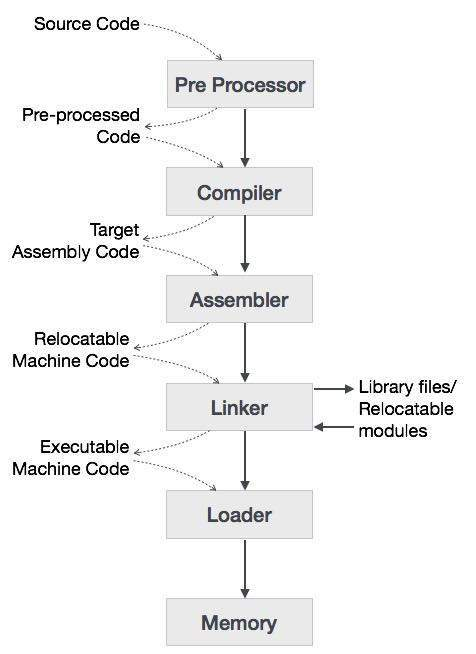
\includegraphics[height=6cm]{img/preprocessor_tricks/language_processing_system.jpg}
    \caption{Language processing system.}
\end{figure}

Let's see the difference in practice. 

\lstinputlisting[language=C,caption={Computing the max (\texttt{src/preprocessor\_tricks/preprocessor\_01.c})}, label={lst:preproc_max}]{src/preprocessor_tricks/preprocessor_01.c}

In Listing \ref{lst:preproc_max}, local variables \texttt{a} and \texttt{b} are mapped to the following stack location in assembly (\texttt{\#} denotes an inline comment):
\begin{verbatim}
mov     DWORD PTR [ebp-12], 0 # a
mov     DWORD PTR [ebp-16], 1 # b
\end{verbatim}
Finding the maximum by calling the macro \texttt{MAX} simply adds more branches to the generated code. The C line below:
\begin{verbatim}
int c = MAX(a, b);
\end{verbatim}
generates the following code:
\begin{verbatim}
    mov     eax, DWORD PTR [ebp-12]
    cmp     eax, DWORD PTR [ebp-16]
    jle     .L6
    mov     eax, DWORD PTR [ebp-12]
    jmp     .L7
.L6:
    mov     eax, DWORD PTR [ebp-16]
.L7:
    mov     DWORD PTR [ebp-20], eax
\end{verbatim}
This is translated into the following pseudocode, where \texttt{[...]} denote memory location:
\begin{verbatim}
    [ebp=12] = 0 # a
    [ebp-16] = 1 # b
    eax = a
    if eax <= b:
        goto .L6
    goto .L7

.L6:
    eax = b
.L7
    [ebp-20] = eax # address ebp-20 stores c
\end{verbatim}
On the other hand, calling the \texttt{max} function:
\begin{verbatim}
int d = max(a, b);
\end{verbatim}
requires pushing the local variables \texttt{a}, \texttt{b} in the stack before the function is called and then popping (\texttt{add esp, 4} pops 4 bytes - one integer) the stack:
\begin{verbatim}
    mov     DWORD PTR [ebp-20], eax
    push    DWORD PTR [ebp-16]
    push    DWORD PTR [ebp-12]
    call    max(int, int)
    add     esp, 8
    mov     DWORD PTR [ebp-24], eax
\end{verbatim}


\subsection{The double evaluation problem of macros}

Passing expressions to macros, such as the output of function, e.g. \texttt{foo()} may hinder the performance of the code due to double evaluation.

\begin{takeaway}[double evaluation problem of macros]
% ref https://stackoverflow.com/questions/39439181/what-is-double-evaluation-and-why-should-it-be-avoided
Passing an expression as an argument to a function-like macro will potentially evaluate that expression twice. That is because the expression will be repeated where ever the macro parameter it takes on, is used in the macro's definition.
\end{takeaway}
This can be remedied by passing values into the macro.

Supposed we have defined a macro for the maximum of two numbers and we want to evaluate py calling two functions:

\begin{lstlisting}[language=c]
#include <stdio.h>

#define MAX(a,b) (((a)>(b))?(a):(b))

int x() { puts("x"); return 0; }
int y() { puts("y"); return 1; }

int main() {
    MAX(x(), y());
}
\end{lstlisting}
\texttt{MAX} in this case will expand to:
\begin{verbatim}
 #define MAX(a,b) ((x() > y()) ? x() : y())   
\end{verbatim}
\begin{verbatim}
When running the C code for \texttt{MAX}, \texttt{x(), y()} are both called once at the test condition and the larger one is called once more. As a result, the program prints:
\begin{verbatim}
x
y
y
\end{verbatim}
Obviously the remedy is to store their returns in local variables and pass the local variables in the macro.

\subsection{Multi-line macros}

Before multi-line are defined, it is important to know about control flow statements not followed by curly braces (``naked'' \texttt{if, else, while, for}).

\begin{takeaway}[naked control flow statements]
A control flow statement that is not followed by {} is considered as a block with the next statement that follows it.
\end{takeaway}

For instance:
\begin{verbatim}
if (condition)
	int a = 1; int b = 2;    
\end{verbatim}
is equivalent to:
\begin{verbatim}
if (condition) {
	int a = 1;
}
int b = 2;    
\end{verbatim}

Back to the main problem -- suppose we want to write a multi-line macro, e.g. a \texttt{FOO} function-like macro that subsequently calls two functions \texttt{foo}, \texttt{bar}. 

\textbf{Attempt 1:}

One naive attempt would be the following:

\lstinputlisting[language=C,caption={First attempt for multi-line macro (\texttt{src/preprocessor\_tricks/preprocessor/preprocessor\_tricks\_02.c})}, label={lst:preproc_foobar1}]{src/preprocessor_tricks/preprocessor_tricks_02.c}

This expends the macro to two statements -- \texttt{foo(42)} and \texttt{bar()} and since ``naked'' \texttt{if} is only followed by one statement, \texttt{bar()} will be executed regardless of the condition.

\textbf{Attempt 2:}

One can try wrapping the two statements in curly braces.
\lstinputlisting[language=C,caption={Third attempt for multi-line macro (\texttt{src/preprocessor\_tricks/preprocessor/preprocessor\_tricks\_03.c})}, label={lst:preproc_foobar2}]{src/preprocessor_tricks/preprocessor_tricks_03.c}

This will be expanded to two statements wrapped in curly braces followed by \texttt{;}:
\begin{verbatim}
if (2 + 2 == 4)
	{ foo(42); bar() };
\end{verbatim}
This in an invalid syntax in C so it will not compile.

\textbf{Attempt 4:}

We can try removing the semicolon after the function-line macro \texttt{FOO2(42)} is called to turn this into a valid \texttt{if} statement:

\lstinputlisting[language=C,caption={Fourth attempt for multi-line macro (\texttt{src/preprocessor\_tricks/preprocessor/preprocessor\_tricks\_04.c})}, label={lst:preproc_foobar2}]{src/preprocessor_tricks/preprocessor_tricks_04.c}

It prints:
\begin{verbatim}
foo
bar
\end{verbatim}
This approach works but it's unconventional as C statements are normally followed by semicolon.

\textbf{Attempt 5:}

One way to consistenly define function-line macros that are followed by a semicolon is by wrapping them in a \texttt{do-while} block as follows:

\lstinputlisting[language=C,caption={Fifth attempt for multi-line macro (\texttt{src/preprocessor\_tricks/preprocessor/preprocessor\_tricks\_05.c})}, label={lst:preproc_foobar5}]{src/preprocessor_tricks/preprocessor_tricks_05.c}

The above program prints the desired output:
\begin{verbatim}
foo
bar
\end{verbatim}
The \texttt{do-while} block ensures the commands inside it will be executed only once. Furthermore, \texttt{do-while} as always followed by a semicolon. Threrefore this idiom not only executes multi-line preprocessor commands, but also must be followed by a semicolon, which makes it consistent with other statements such as function calls. For code maintainability purposes, it's a good practice to wrap \textit{any} macro in \texttt{do-while} -- even single-line ones.
\begin{takeaway}[multi-line macros]
To define a multiple statements \texttt{statement1; statement2; ...} in a macro, they can be wrapped in a \texttt{do-while} block as follows:
\begin{verbatim}
#define FOO(arg1, arg2, ...) do { statement1; statement2; ... } while(0)
\end{verbatim}
\end{takeaway}